\clearpage
\section{Software}
\label{sec:software}

\subsection{OS}
As the authors had most experience with Arch Linux and it's environment, we decided to go with the distribution provided by the Arch Linux for ARM project.
The OS is distributed as a ISO image, which is written to the SD card using the UNIX disk utility {\tt dd}:
\begin{lstlisting}
dd if=inputimage.iso of=/dev/outdisk bs=1M
\end{lstlisting}

\subsection{Searching in general}
Since a significant part of our project is related to searching, we find it reasonable to include a section on how a search engine works in general. 

Our engine consist of two parts: indexing and searching. 
The search engine executes and scores a set of documents for given queries. For this work, it uses the dictionary, and a postings file.
The other part is the indexer, which builds an inverted index, the dictionary, and the postings file\cite{IntroIR} over a collection of documents (corpus).

When performing the indexing task, a loop runs over every document in the corpus. 
For every word encountered in a document, the indexer emits a term, which is made into a token. 
A token what is left after post-processing a term. This processing usually includes stemming and removal of special characters. 
The token is added to a dictionary and the document id is appended to the token's postings list. A counter is also kept along with the id to keep track of multiple occurrences of the same token in the same document.
The result of this loop is a dictionary of all unique tokens encountered, along with a postings list, naming all the documents that contain each token.

The dictionary contains the token, how many times it occurs in the collection, and a pointer to where this term is stored in the postings file.
The entries can be viewed as a tuple of the format:
$$<token, count, pointer>$$
The postings pointer is in our case an integer. This integer is the byte offset in the posting file where this terms posting list starts.

The postings entries are a list of tuples, in the format $$<docID, count>$$, giving the document id where the token occurred and the number of times it was seen in that document.

\begin{figure}[h]
    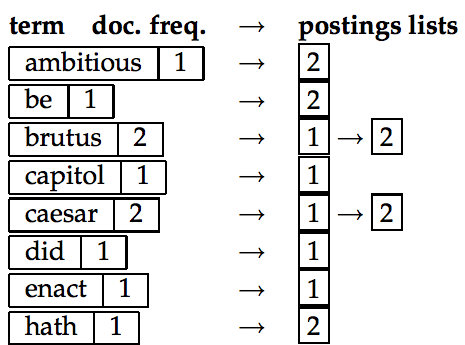
\includegraphics[width=0.5\textwidth]{software/index_postings_lists}
    \center
    \caption{A sample index and postings list.\cite{IntroIR}}
    \label{fig:index_postings_lists_sw}
\end{figure}

\subsection{Document scoring}
In the searching step one is usually working with a query containing one or more terms. For each token the corresponding postings list is fetched from disk (and cached). Each document is then scored according to a scoring scheme and a list of the documents sorted by the score is returned to the application.

To provide a rudimentary form of scoring, we have implemented the TF-IDF scoring system for queries. We are using the weighting scheme suggested by Introduction to Information Retrieval\cite{IntroIR}, {\tt lnc.ltc} in SMART notation\cite{tfidfsmart}.


\subsection{Operating system and environment} % TODO: remove this?

\subsection{Load generator}
The purpose of the load generator is to generate pseudo-random queries and send these to the load distributor to simulate load on the cluster. These queries are of varying length and contains a subset of the tokens found in the dictionary. It also includes some tokens not found in the dictionary.

The load generator runs on several threads, where one thread is responsible for receiving answers for the queries, and one or more threads are responsible for generating load for the system. The load generator is implemented in python and meant to be run on a node outside the cluster.

The load generator includes some configurable parameters, most importantly the frequency of the queries being sent and the number of threads sending queries simultaneously.

\subsection{Load distribution}
One of the nodes in the cluster will be in charge of load distribution. The load distributor node will receive all the queries and then forward them to the worker nodes.
The node employs the very simple load balancing scheme of $$rand() \bmod N,$$ where N is the number of nodes in the cluster.
The messages from the load distributor to the worker nodes includes information of where to deliver the search results when they are ready.
This scheme is simple, but could also prove to be a bottleneck of the system. Seeing as all communication has to go through this node we could end up with the performance of the cluster being limited by the load distributor.

\subsection{Original python version}
The python version we were basing the program on relied heavily upon the python library Natural Language Toolkit\cite{nltk} (NLTK).
NLTK provides a lot of useful methods for processing natural languages in Python, including different tools for stemming and other tokenization tricks.
Stemming is the process of reducing inflected or conjugated words into their basic or root form. Examples include removal of prefixes, suffixes, tense and vowel changes. I.e. words like ``fishing'', ``fisher'' and ``fished'' all end up mapping to the same stem ``fish''.

The toolkit also provides stop word lists and improved splicing of natural language sentences. As this is a lot of work to implement, we have chosen to do indexing in python and deliver and calculate search results based only on the stemmed forms for the C program.

\subsection{Optimized C-port}
In practice we experienced serious performance issues with our python code, often showing response times in the hundreds of milliseconds. We therefore decided to rewrite the program using C. This proved it both challenging and useful to control what exactly is present in memory at every moment, in addition to the extra work of having to control memory allocation.

The program reads the dictionary structure into memory on startup. It provides O(1) lookup on query terms in a hash map, using the library {\tt uthash}\cite{uthash}.

\begin{lstlisting}[style=customc,captionpos=b,caption={Structure of a dictionary entry (term)}]
typedef struct {
    char* term;
    uint32_t byte_offset;
    uint32_t occurences;
    postings_entry* posting;
    UT_hash_handle hhd;         /* makes this structure hashable */
} dictionary_entry;
\end{lstlisting}
\subsubsection{uthash}
{\tt uthash} is a small library with a set of convenient preprocessor macros for creating and managing hash tables in C. 
{\tt uthash} does constant time $$O(1)$$ lookups, inserts and deletes, and comes with a number of different hash functions in case your key domain is not well suited for the default hash function. 

\subsubsection{Experiences}
The first testings of the C-port showed significant improvements in delivery speed.
It further confirmed that managing memory yourself is desirable for performance, and is especially important in an environment where resources are scarce. 
When blasting the searching code with queries, we quickly maxed out the available memory.
These memory leaks were later fixed, and the program now experiences constant memory usage. The difference in developing platform, compared to the ARMv6 runtime environment did not impose any extra difficulties, except for a single case of some odd pointer behavior.
The rest of the time, the code behaved as expected from one platform to the other.

For comparison between the two languages, we created a test set of 100,000 queries. We then ran this test set against the reference MacBook computer, and on the pi, both for Python and {C}. 
The results are given in Table \ref{tbl:runtimes_ports}. 

For the relatively quick {Core i5}, the python code need 10 times longer to run the queries than the C code, and seem reasonable compared to known sources.
The Python code is however detrimental to the performance for the weaker PI. The same 100,000 queries takes 84 seconds to run in C, but takes 24 times longer in python.

\begin{table}[h]
	\begin{center}
	\begin{tabular}{|r|r|r|}
	\hline
	   & \multicolumn{1}{|c|}{PI}     & \multicolumn{1}{|c|}{MacBook} \\
	\hline
	C      & 84.748   & 4.782     \\
	\hline
	Python & 2046.768 & 49.411    \\
	\hline
	\end{tabular}
	\caption{Runtimes (in seconds) for C and Python code on 100,000 queries.}
	\label{tbl:runtimes_ports}
	\end{center}
\end{table}
